\documentclass[11pt, a4paper, oneside]{article}


\usepackage[margin=1.5cm]{geometry}
\usepackage{graphicx} %Pretty documents
\usepackage{grffile} %Allow multi-dots in image names (otherwise first dot seen as file extention)
\graphicspath{{./tex_images/}}
\usepackage{parskip} %No Indentation for Paragraphs
\usepackage[hidelinks]{hyperref} %Clickable PDF's
\usepackage{blindtext} %Use for text fillers and formatting
\usepackage{float} %Allow H in figures to fix position
\usepackage{siunitx} %Propper SI Units \SI{Value}{Units}
\usepackage{caption} %Allows caption*() to remove prefix for equations in figures
\usepackage{listings} %code
\usepackage{verbatim}
\usepackage{booktabs}
\usepackage{textcomp}
\usepackage{courier}
\usepackage{caption}
\usepackage{subcaption}

\lstset{basicstyle=\footnotesize\ttfamily,breaklines=true}
\lstset{framextopmargin=50pt,frame=bottomline}

\begin{document}
	
	\noindent
\begin{center}
	\includegraphics[width=\columnwidth]{tudelftlogo.eps} \\
	
	\large{EE2T11 - Telecommunications Practical}\\
	\begin{LARGE}
		\textbf{Midterm Report - Group A24} \\[0.3cm]
	\end{LARGE}
	\today \\[.2cm]
	\begin{tabular}{l l} \\
		Nicolaas du Plessis & 4203933 \\
		
	\end{tabular}
\end{center}

\newpage
		\section*{1: Convolution}
	\subsection*{Report 1}

	A step and impulse response was convoluted with a transfer function of a high pass and low pass filter, with coefficient "a" being 0.95 and -0.95 for each respective filter. The MATLAB script used can be found on page \pageref{matlab_1.1}. The original input signals can be seen below in figure \ref{figure:1_1_1}. N was chosen as 100 samples, as the increased resolution gives a better indication on the nature of the responses.
	
	\begin{figure}[H] 
		\centering
		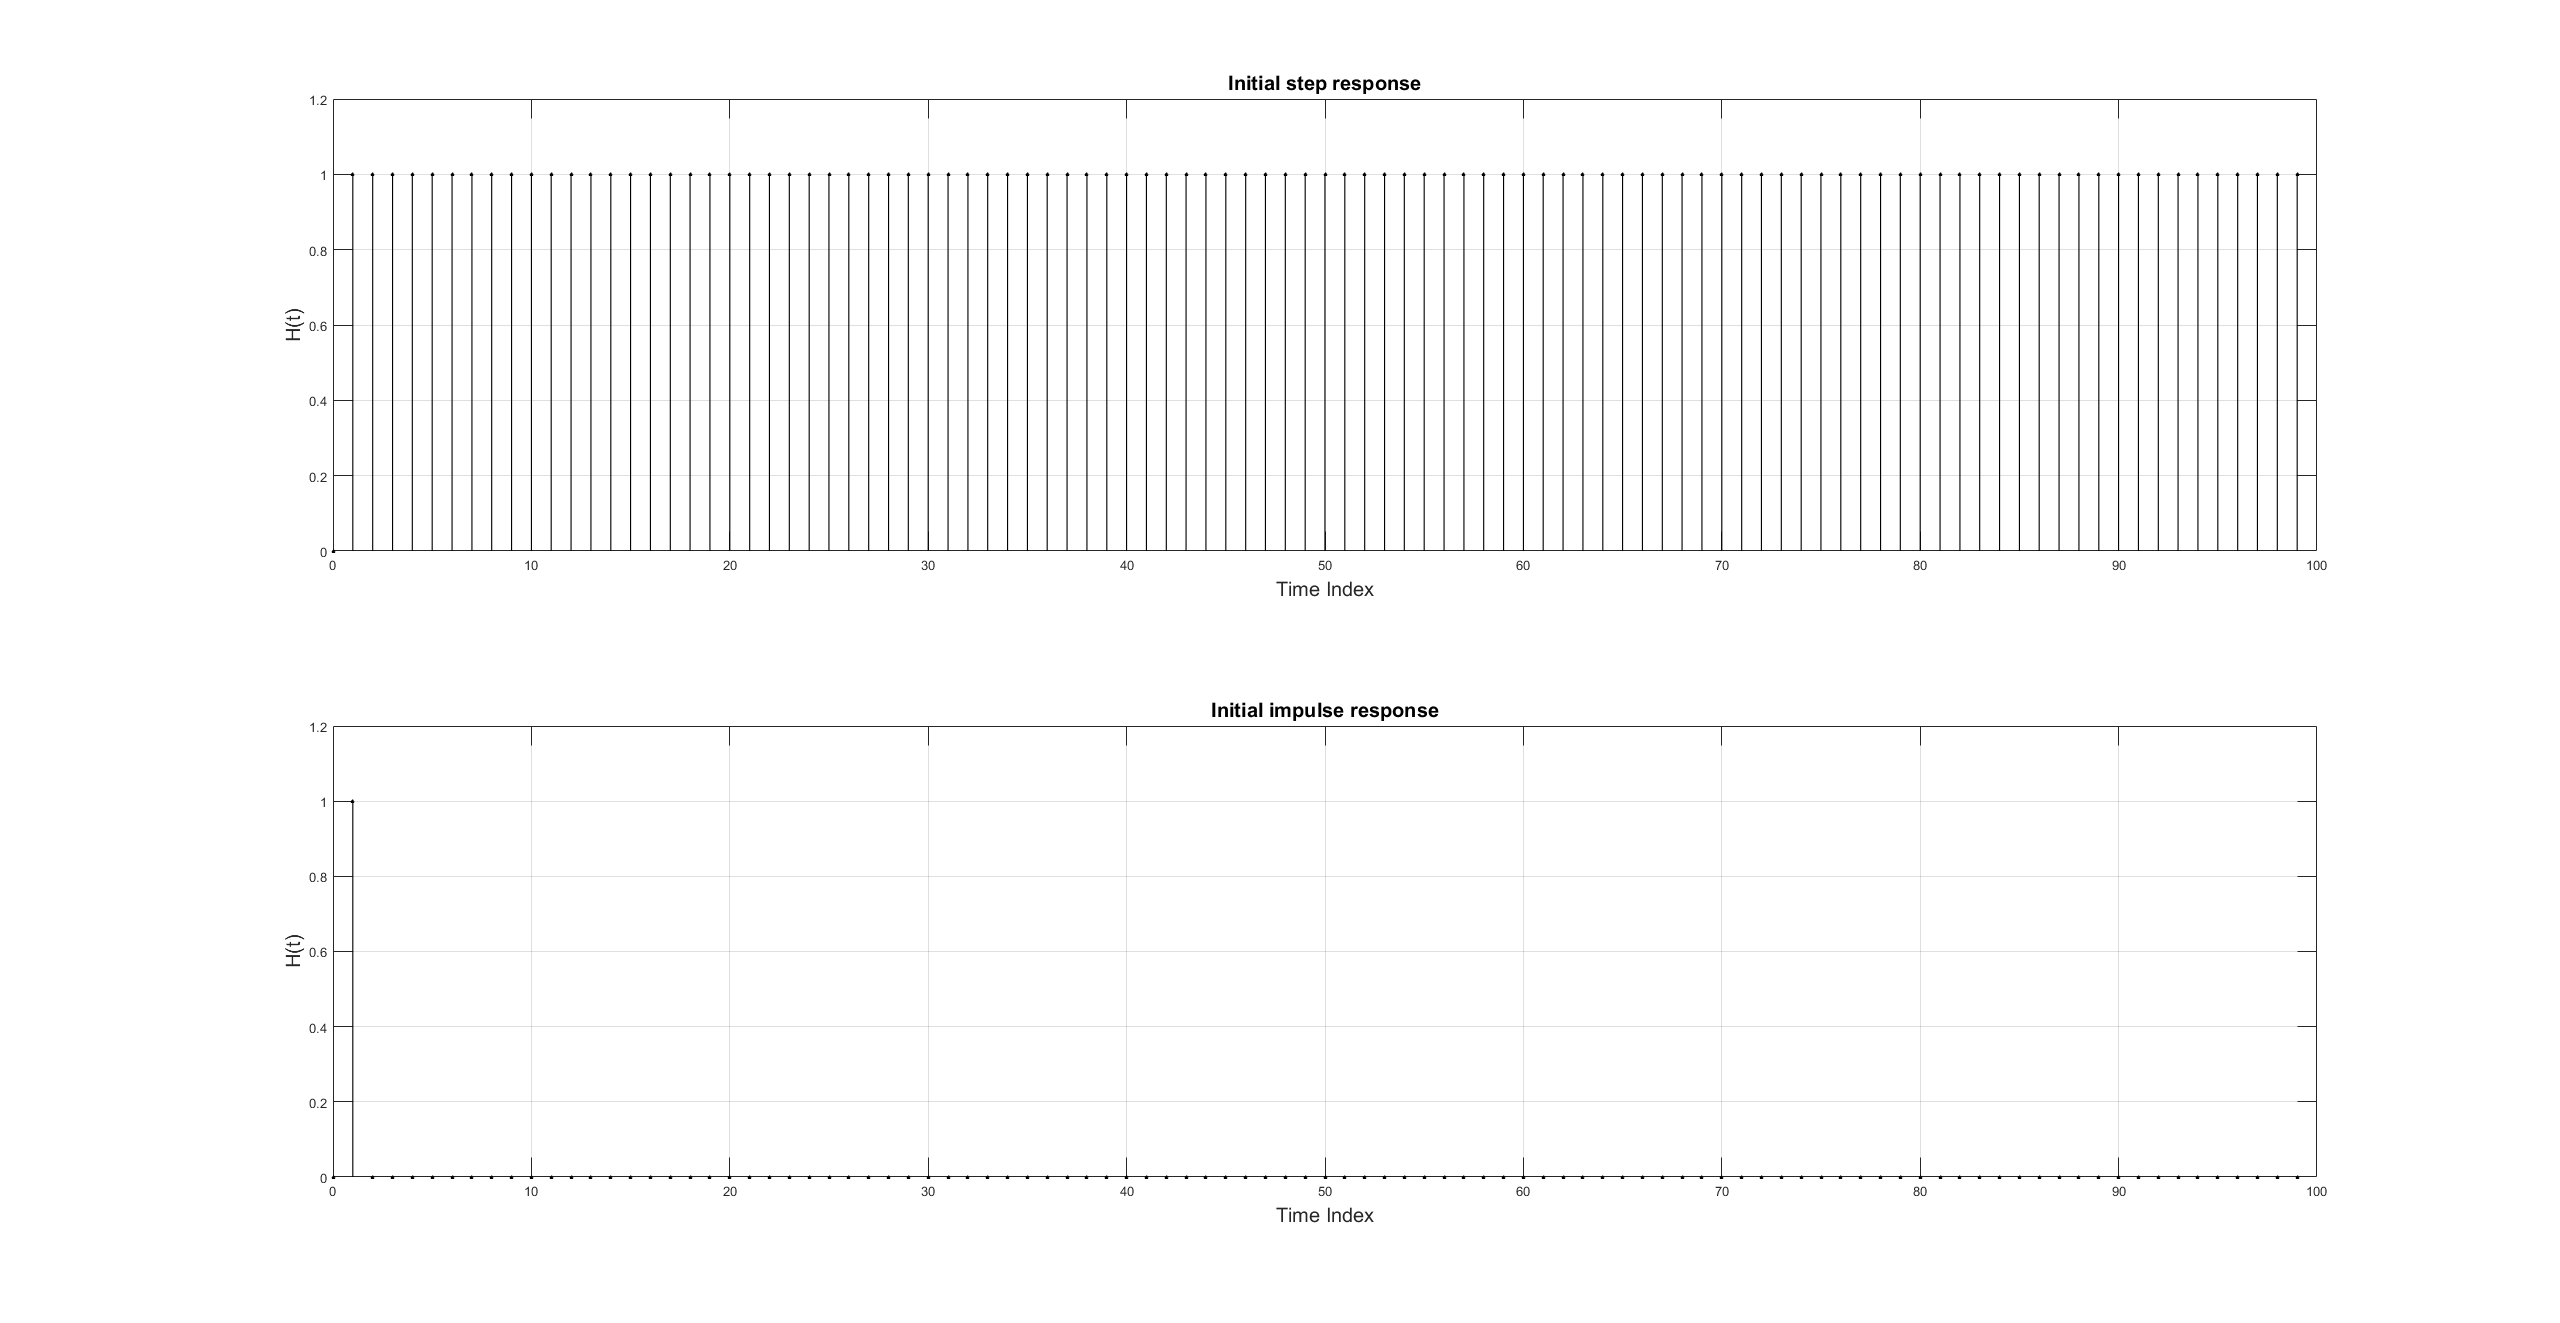
\includegraphics[width=\textwidth]{1.1.1.png}
		\caption{Input Impulse and Step Response}
		\label{figure:1_1_1}
	\end{figure}
	
	For the low pass signal response as seen in figure \ref{figure:1_1_2}, the step response (which contains very high frequency components) in filtered, which only leaves the low frequecy components, meaning the filter takes a while to equalize (reach the input value), which is typical of a low pass filter. Similarly, the impulse response shows the effective settling time of the filter after an impulse, dependant on the filter coefficient.
	
	\begin{figure}[H] 
		\centering
		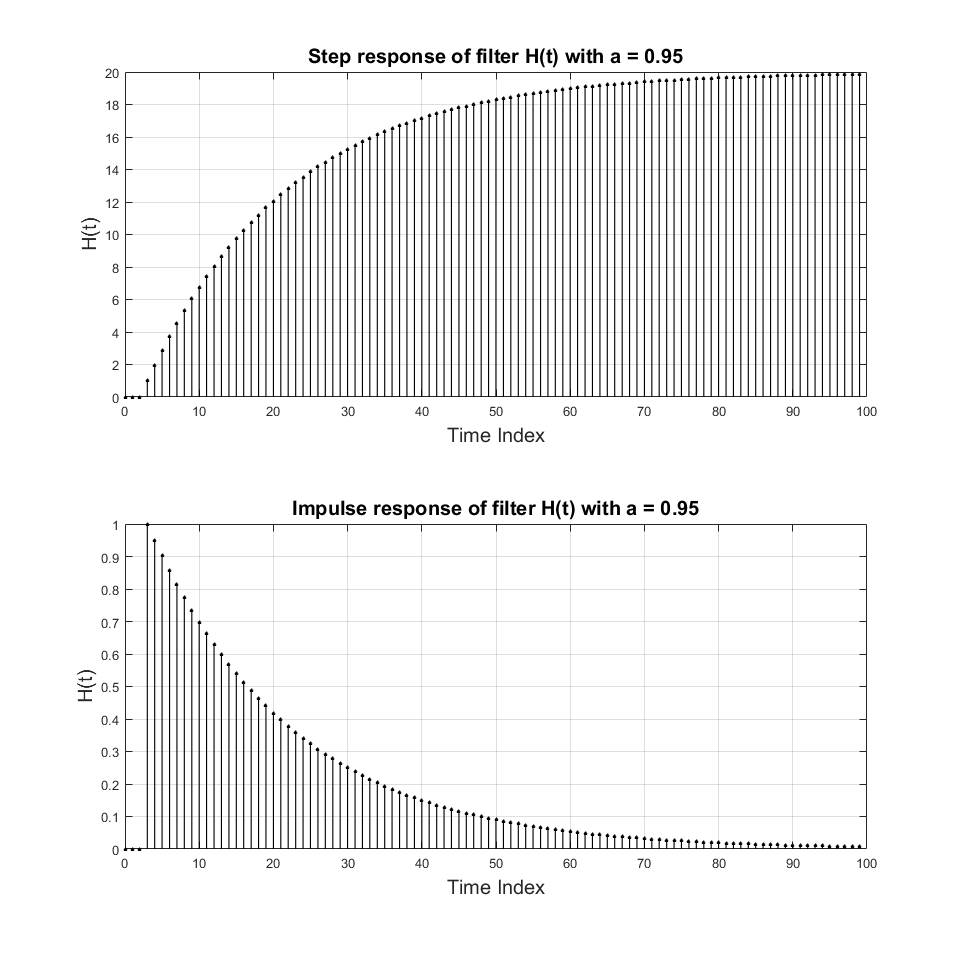
\includegraphics[width=\textwidth]{1.1.2.png}
		\caption{Low Pass Filter Response with a=0.95}
		\label{figure:1_1_2}
	\end{figure}

	For the high pass signal response as seen in figure \ref{figure:1_1_3}, the difference in amplitude for the step response is magnified greatly, as the high frequency content of the filter allows for the quick rise time. However, as these frequencies are not dampened by the filter, they dent to oscillate, which can also be seen in the figure. The impulse signal results as shows an oscillatory behaviour, as the high frequency components of the impulse are greatly magnified, but not dampened.
	
	\begin{figure}[H] 
		\centering
		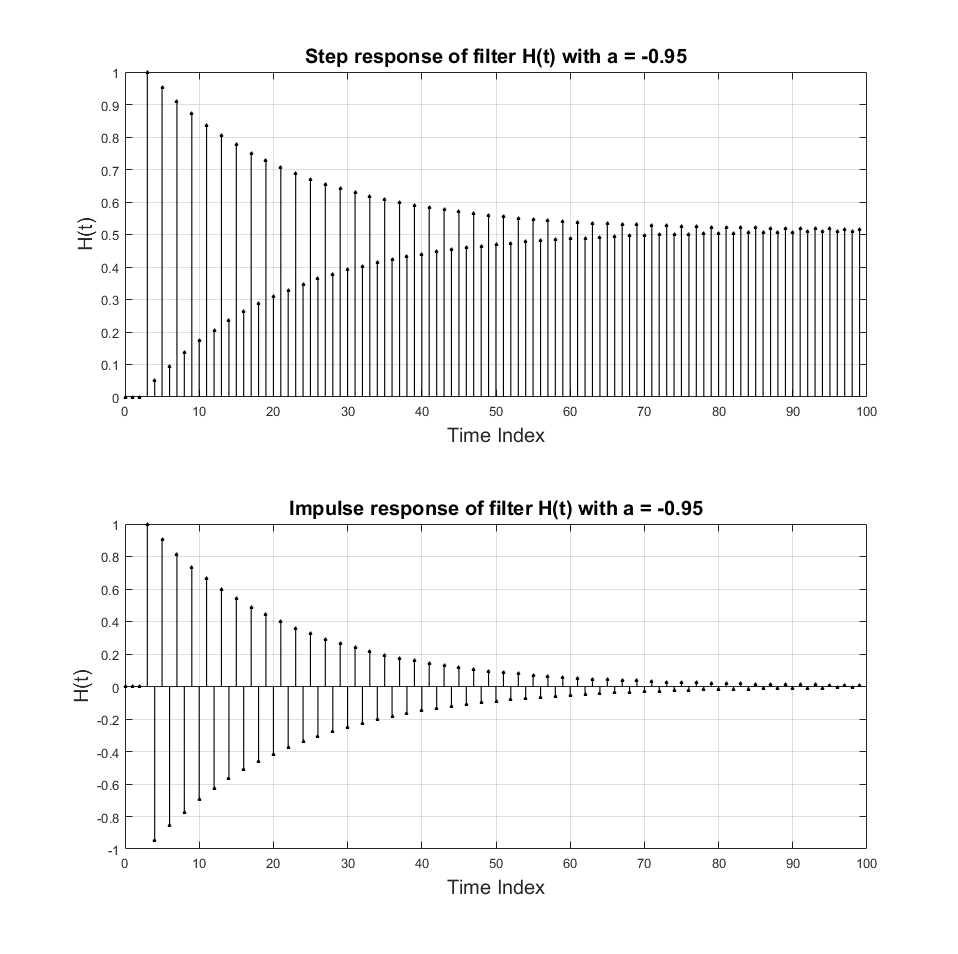
\includegraphics[width=\textwidth]{1.1.3.png}
		\caption{High Pass Filter Response with a=-0.95}
		\label{figure:1_1_3}
	\end{figure}
	\subsection*{Report 2}

	The second exercise simulated sound travelling from a source to a target, with first and second order reflections from the walls being included. The MATLAB script used can be found on page \pageref{matlab_1.2}. A damping factor of 0.5 was used to allow the signals to decrease over time, as it would in reality. An impulse response was sent as the source, and from the simulated received pulses the room channel impulse response was calculated through a convolution of the original impulse response and the simulated received response. Figure \ref{figure:1_2} shows that both the received signal and calculated response are the same, as expected.
	
	\begin{figure}[H] 
		\centering
		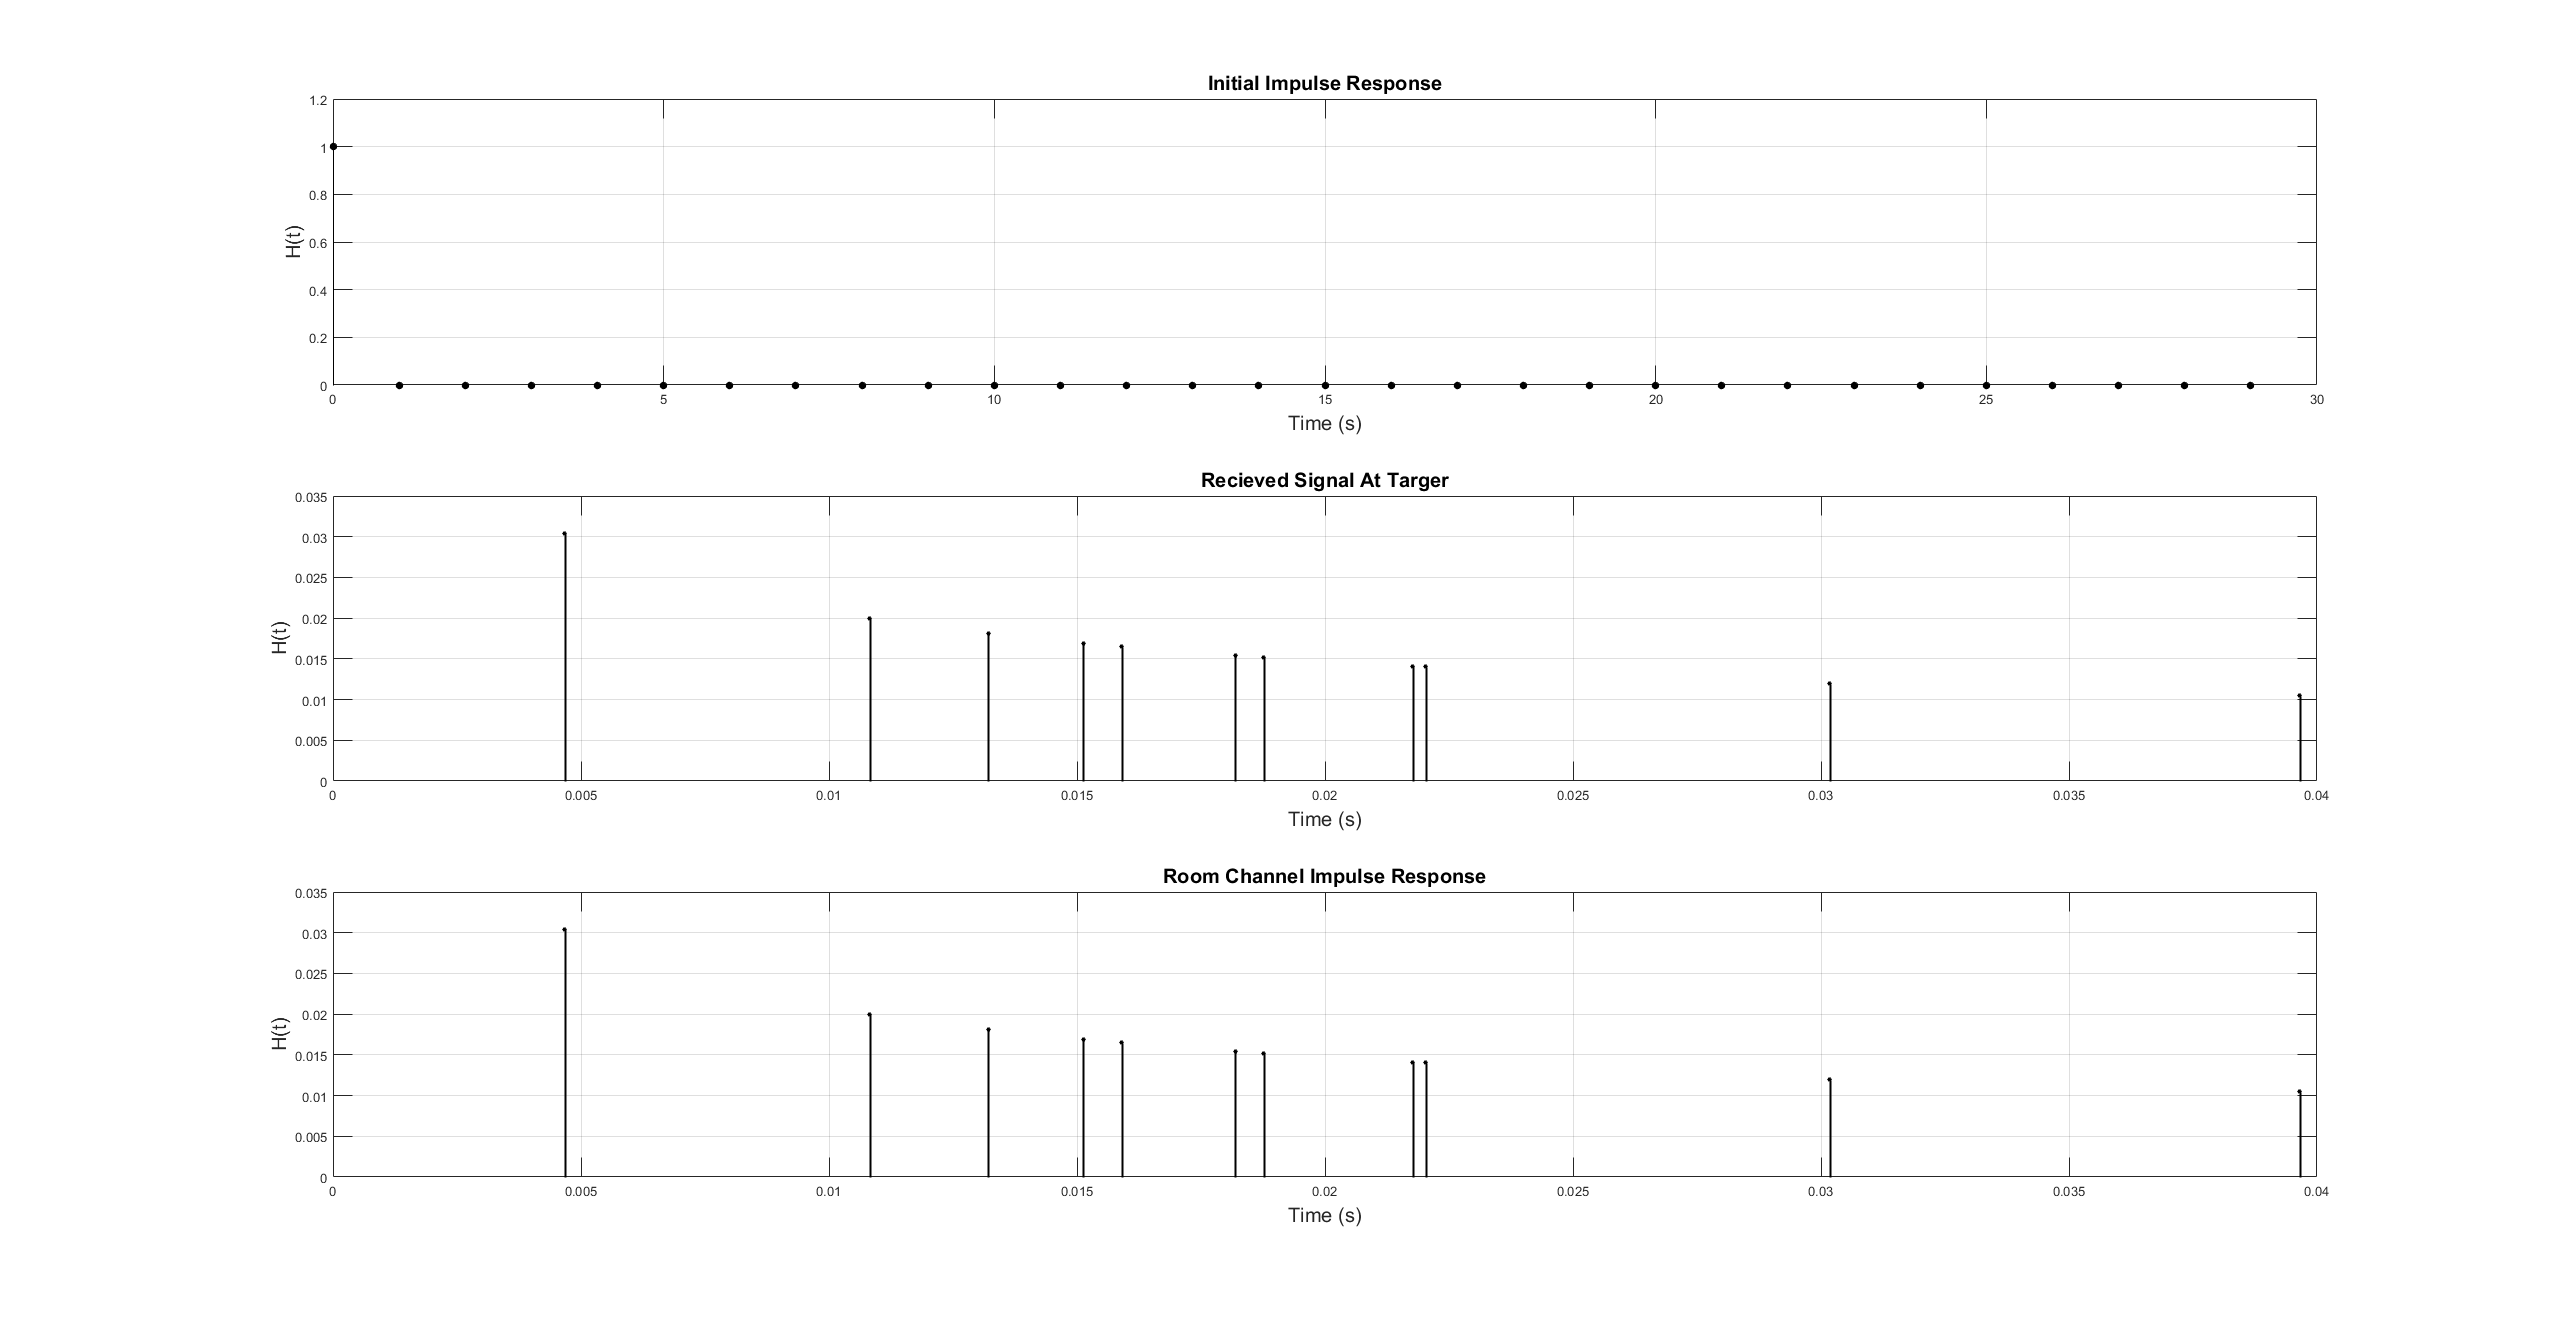
\includegraphics[width=\textwidth]{1.2.png}
		\caption{Room Channel Impulse Response \& Reflected Signals}
		\label{figure:1_2}
	\end{figure}
		\section*{2: Fourier Transformation}
	\subsection*{Report 3}

	In figure \ref{figure:2_1}, time and frequency domain plots of three audio signals are shown. The frequency domain plots where obtained using the MATLAB function \verb+fft+. The frequency spectrum is symmetrical around the DC component $f = 0 \si{\hertz}$. The symmetry is a result of the discrete fourier transform, which is complex conjugate symmetric. Plotting only the positive frequencies would be a logical choice, since no information is lost. The used MATLAB script can be found on page \pageref{matlab_2.1}.

	\begin{figure}[H] 
		\centering
		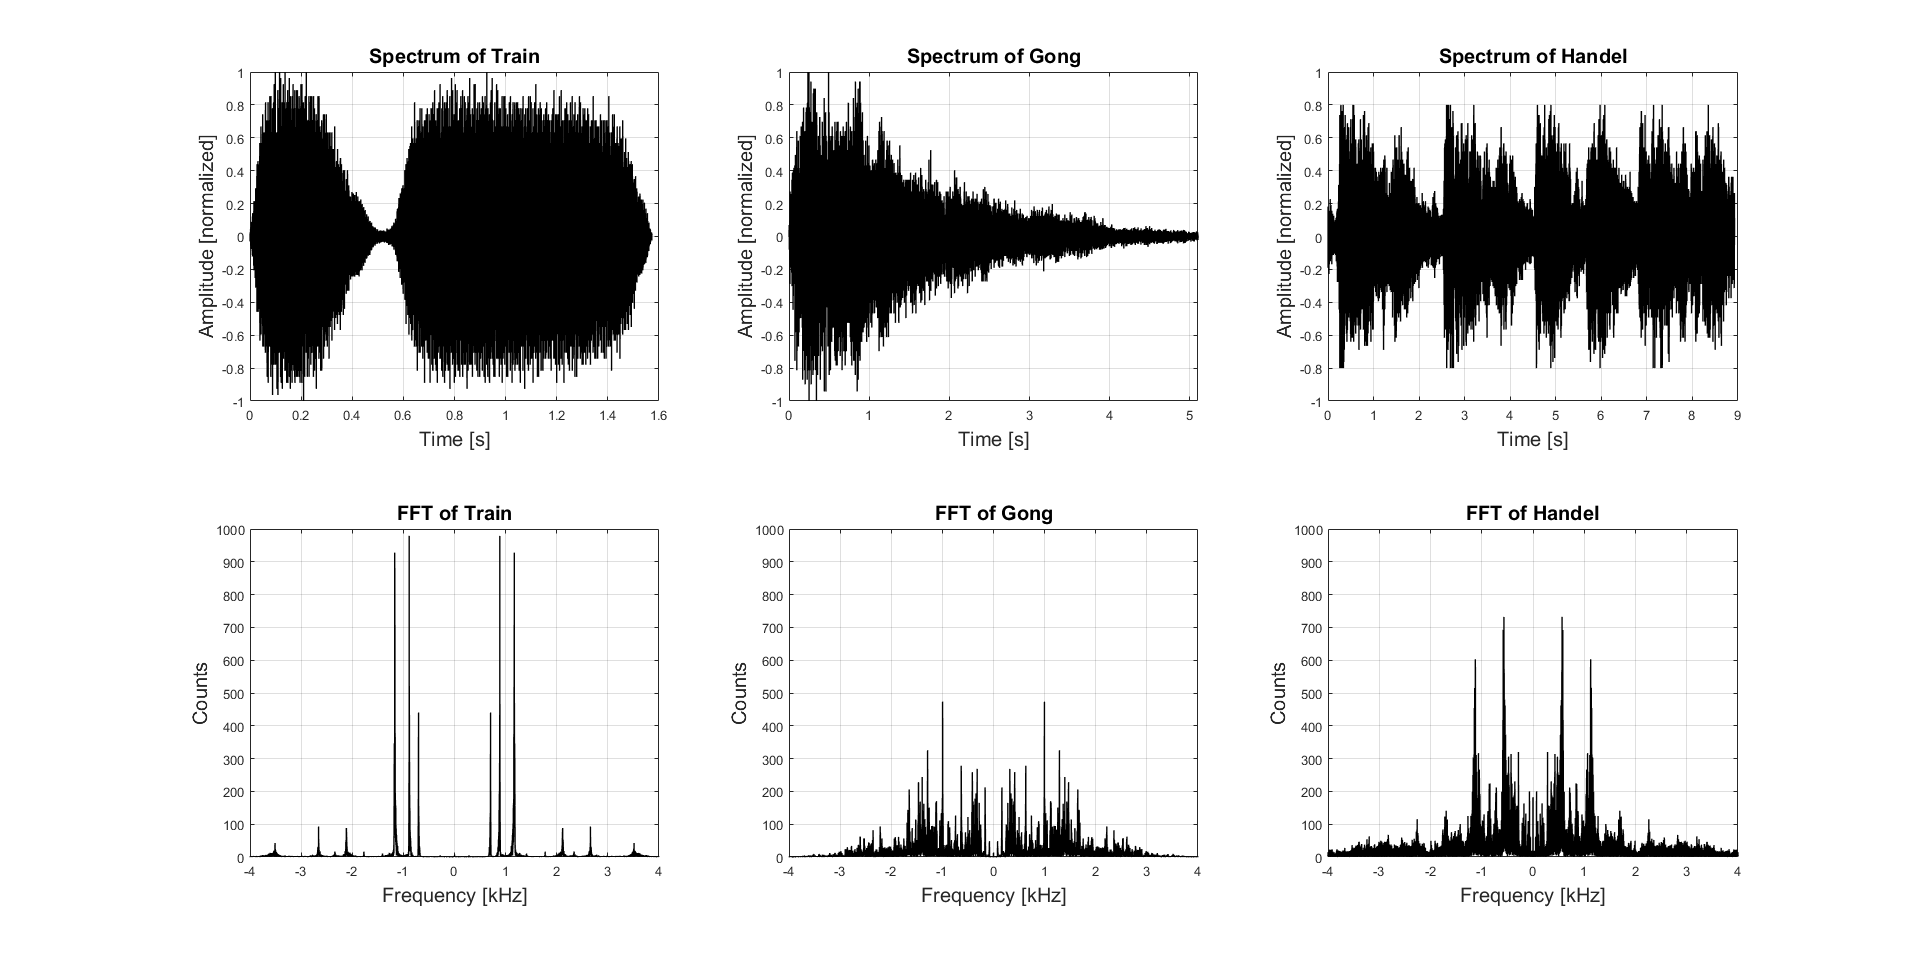
\includegraphics[width=\textwidth]{2.1.png}
		\caption{Time Domain \& Frequency Domain plots of standard MATLAB sounds}
		\label{figure:2_1}
	\end{figure}

		
	\subsection*{Report 4}

In figure \ref{figure:2_2} the train signal is reshaped into segments of 20ms, and afterwards the DFT is applied to each segment. Enlarging the segment size will give a better resolution on the frequency axis, but lower on the time axis. The opposite is also true: smaller segment size gives a better time resolution, but worse frequency resolution. This plot is more useful than the non-segmented plot in figure \ref{figure:2_1} since variations in time in the signal are now visible.
	\begin{figure}[H] 
		\centering
		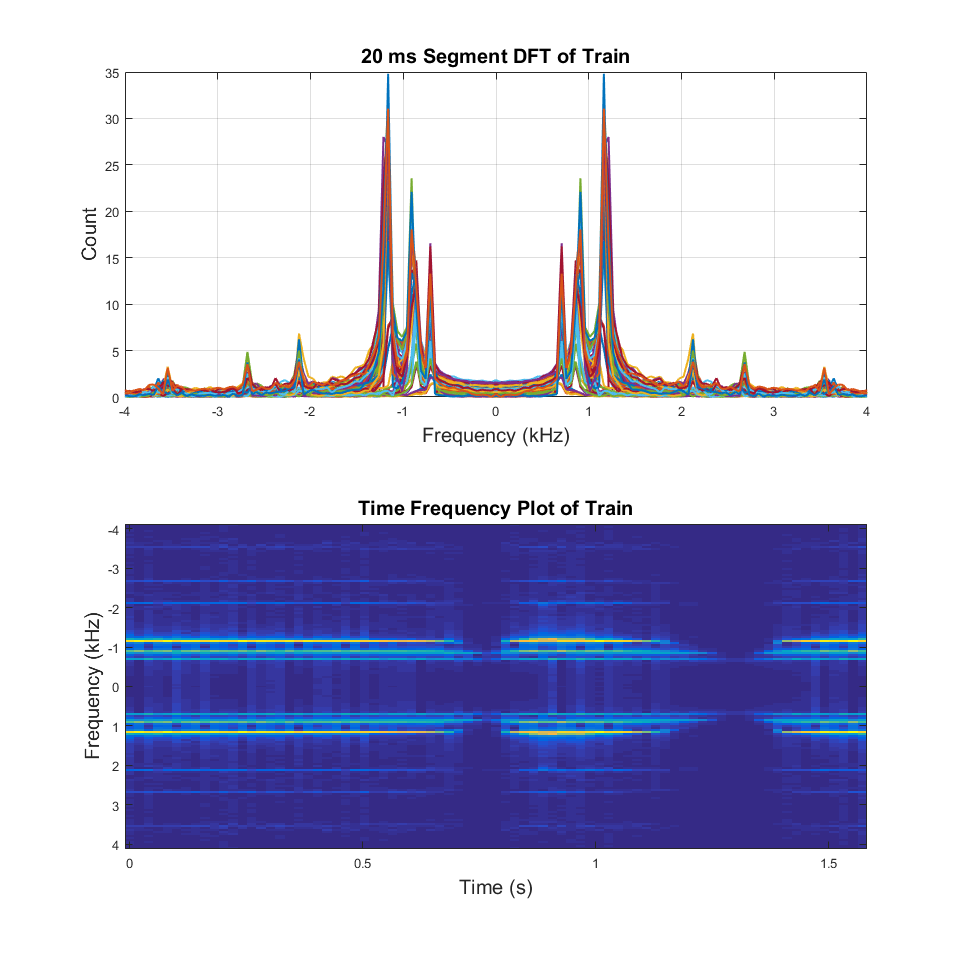
\includegraphics[width=\textwidth]{2.2.png}
		\caption{Train - Segmented FFT \& Time Frequency Plot}
		\label{figure:2_2}
	\end{figure}
	
	
		\subsection*{Report 5 + 6}
	When the sample size is small, the resolution of corresponding FFT is limited as demonstrated in the previous report. If the time domain signal is zero-padded, the longer time signal will yield an interpolated signal in the frequency domain. This effect is shown below in figure \ref{figure:2_3}, where the original signal and zero padded signal show the clear interpolation that occurs as a result of zero padding. The MATLAB script that was used can be found on page \pageref{matlab_2.3}.
	
	\begin{figure}[H] 
		\centering
		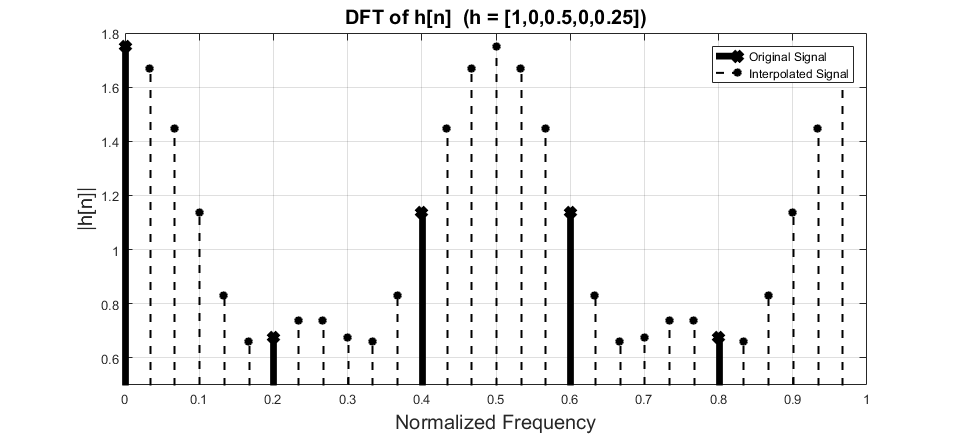
\includegraphics[width=\textwidth]{2.3.png}
		\caption{Interpolated sequence with DFT through zero padding}
		\label{figure:2_3}
	\end{figure}
	\subsection*{Report 7}
In figure \ref{figure:2_4}, the result of the convolution with the train audio signal $x$ and the filter $h$ is shown. Both plots are identical, indicating that the convolution $ y[n] = x[n] \ast h[n] $ can be archived using the property $ Y(\omega) = X(\omega) H(\omega) $.

	\begin{figure}[H] 
		\centering
		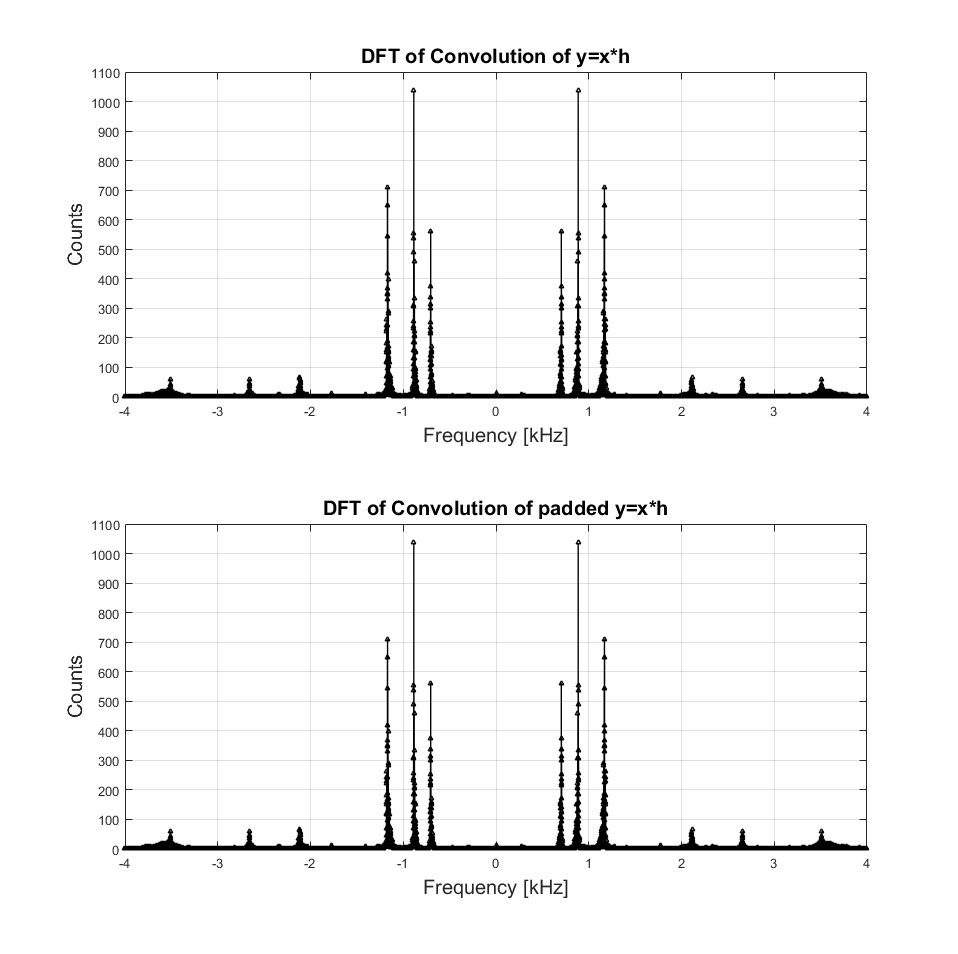
\includegraphics[width=\textwidth]{2.4.png}
		\caption{Comparison of DFT of convolution for original and padded signals}
		\label{figure:2_4}
	\end{figure}
	
	%\input{tex_sections/report_8.tex}

	%\section*{3: Channel Estimation}
	%\input{tex_sections/report_9.tex}
	%\input{tex_sections/report_10.tex}
	%\input{tex_sections/report_11.tex}
	%\input{tex_sections/report_12.tex}

	%\section*{4: Audio Channel Measurement}
	%\input{tex_sections/report_13.tex}
	%\input{tex_sections/report_14.tex}
	%\input{tex_sections/report_15.tex}
	%\input{tex_sections/report_16.tex}
	%\input{tex_sections/report_17.tex}

	%\section*{5: Filter Design}
	%\input{tex_sections/report_18.tex}
	%\input{tex_sections/report_19.tex}
	%input{tex_sections/report_20.tex}
	%\input{tex_sections/report_21.tex}
	%\input{tex_sections/report_22.tex}
	%\input{tex_sections/report_23.tex}
	%\input{tex_sections/report_24.tex}

	%\section*{6: Sampling}
	%\input{tex_sections/report_25.tex}
	%\input{tex_sections/report_26.tex}
	%\input{tex_sections/report_27.tex}
	%\input{tex_sections/report_28.tex}
	%\input{tex_sections/report_29.tex}
\newpage
	\section*{Appendix: Matlab Scripts}
		%\lstset{language=Matlab,upquote=true}
	
	\subsection*{Script for Report 1} \label{matlab_1.1}
	\lstinputlisting[language=Matlab, breaklines=true]{scripts_report/code1_1.m}
	\subsection*{Script for Report 2} \label{matlab_1.2}
	\lstinputlisting[language=Matlab, breaklines=true]{scripts_report/code1_2.m}
	
	\subsection*{Script for Report 3} \label{matlab_2.1}
	\lstinputlisting[language=Matlab, breaklines=true]{scripts_report/code2_1.m}
	\subsection*{Script for Report 4} \label{matlab_2.2}
	\lstinputlisting[language=Matlab, breaklines=true]{scripts_report/code2_2.m}
	\subsection*{Script for Report 5+6} \label{matlab_2.3}
	\lstinputlisting[language=Matlab, breaklines=true]{scripts_report/code2_3.m}
	\subsection*{Script for Report 7} \label{matlab_2.4}
	\lstinputlisting[language=Matlab, breaklines=true]{scripts_report/code2_4.m}
	%\subsection*{Script for 2.5} \label{matlab_2.5}
	%\lstinputlisting[language=Matlab, breaklines=true]{scripts_report/code2_5.m}
	
	%\subsection*{Script for 3.1} \label{matlab_3.1}
	%\lstinputlisting[language=Matlab, breaklines=true]{scripts_report/code3_1.m}
	%\subsection*{Script for 3.2} \label{matlab_3.2}
	%\lstinputlisting[language=Matlab, breaklines=true]{scripts_report/code3_2.m}
	%\subsection*{Script for 3.3} \label{matlab_3.3}
	%\lstinputlisting[language=Matlab, breaklines=true]{scripts_report/code3_3.m}
	%\subsection*{Script for 3.4} \label{matlab_3.4}
	%\lstinputlisting[language=Matlab, breaklines=true]{scripts_report/code3_4.m}
	%\subsection*{Script for 3.5} \label{matlab_3.5}
	%\lstinputlisting[language=Matlab, breaklines=true]{scripts_report/code3_5.m}
	%\subsection*{Script for 3.6} \label{matlab_3.6}
	%\lstinputlisting[language=Matlab, breaklines=true]{scripts_report/code3_6.m}
	%\subsection*{Script for 3.7} \label{matlab_3.7}
	%\lstinputlisting[language=Matlab, breaklines=true]{scripts_report/code3_7.m}
		
	%\subsection*{Script for 4.1} \label{matlab_4.1}
	%\lstinputlisting[language=Matlab, breaklines=true]{scripts_report/code4_1.m}
	%\subsection*{Script for 4.2} \label{matlab_4.2}
	%\lstinputlisting[language=Matlab, breaklines=true]{scripts_report/code4_2.m}
	%\subsection*{Script for 4.3} \label{matlab_4.3}
	%\lstinputlisting[language=Matlab, breaklines=true]{scripts_report/code4_3.m}
	%\subsection*{Script for 4.4} \label{matlab_4.4}
	%\lstinputlisting[language=Matlab, breaklines=true]{scripts_report/code4_4.m}
	%\subsection*{Script for 4.5} \label{matlab_4.5}
	%\lstinputlisting[language=Matlab, breaklines=true]{scripts_report/code4_5.m}
	
	%\subsection*{Script for report 18} \label{matlab_18}
	%\lstinputlisting[language=Matlab, breaklines=true]{scripts_report/Report18.m}
	%\subsection*{Script for report 19} \label{matlab_19}
	%\lstinputlisting[language=Matlab, breaklines=true]{scripts_report/Report19.m}
	%\subsection*{Script for report 20} \label{matlab_20}
	%\lstinputlisting[language=Matlab, breaklines=true]{scripts_report/Report20.m}
	%\subsection*{Script for report 21} \label{matlab_21}
	%\lstinputlisting[language=Matlab, breaklines=true]{scripts_report/Report21.m}
	%\subsection*{Script for report 23} \label{matlab_23}
	%\lstinputlisting[language=Matlab, breaklines=true]{scripts_report/Report23.m}
	%\subsection*{Script for report 24} \label{matlab_24}
	%\lstinputlisting[language=Matlab, breaklines=true]{scripts_report/Report24.m}
	%\subsection*{Script for report 25} \label{matlab_25}
	%\lstinputlisting[language=Matlab, breaklines=true]{scripts_report/Report25.m}
	%\subsection*{Script for report 26} \label{matlab_26}
	%\lstinputlisting[language=Matlab, breaklines=true]{scripts_report/Report26.m}
	%\subsection*{Script for report 27} \label{matlab_27}
	%\lstinputlisting[language=Matlab, breaklines=true]{scripts_report/Report27.m}
	%\subsection*{Script for report 28 and 29} \label{matlab_28}
	%\lstinputlisting[language=Matlab, breaklines=true]{scripts_report/Report28.m}

\end{document}
